%!TEX TS-program = xelatex
%!TEX encoding = UTF-8 Unicode
\documentclass[11pt, parindent=0]{article} % use larger type; default would be 10pt
\sloppy

%----------------------------------------------------------------------------------------
%   PACKAGES
%----------------------------------------------------------------------------------------
\usepackage{afterpage}
%\usepackage[demo]{graphicx} % support the \includegraphics command and options
\usepackage{graphicx}
\usepackage[parfill]{parskip}
\usepackage{hyperref}
\usepackage{amsmath,amsfonts,amsthm} % Math packages
\usepackage{mathtools}
\usepackage{relsize} % for mathlarger
\usepackage{lipsum} % Used for inserting dummy 'Lorem ipsum' text into the template
\usepackage{datetime}
\usepackage{xfrac}
\usepackage{changepage} % for adjusting the width
\usepackage{gensymb}
\usepackage{subcaption}
\usepackage{sectsty}
\usepackage{xcolor}
\usepackage{verbatim}
\usepackage{titlesec}
% not needed in >2015 versions
%\usepackage{fixltx2e} %helps the [H] problem! 10/2/2015
\usepackage{color}
\usepackage{float} % Not have your figures fly around  - use [H]
\usepackage{booktabs} % for much better looking tables
\usepackage{array} % for better arrays (e.g matrices) in maths
\usepackage{paralist} % very flexible & customisable lists (eg. enumerate/itemize, etc.)
\usepackage{verbatim} % adds environment for commenting out blocks of text & for better verbatim
\usepackage[export]{adjustbox}
\usepackage{pdfpages} % For pdf inputs
\usepackage{import} % for subfolder inputs
\usepackage{metalogo} % for the fucking logo
\usepackage{listings}
\usepackage{mdwlist} % for tight lists
\usepackage{letltxmacro} % better roots
\usepackage{xspace} % for correct spacing
\usepackage{multicol} % for the multicol environment
\usepackage{wrapfig}
\usepackage{tabularx}
\usepackage{nomencl}
\usepackage[noabbrev]{cleveref}      % reference object types automatically
\usepackage{mathrsfs} % for fancy F symbol

% mediocre solution - fixing the quotes problem
\usepackage [autostyle]{csquotes}
\MakeOuterQuote{"}

% underlining with color
\usepackage{soul}
\setul{}{2pt}
\definecolor{yellow}{rgb}{1.0, 0.8, 0}
\setulcolor{yellow}


\makenomenclature %change position

%----------------------------------------------------------------------------------------
%   DOCUMENT CONFIGURATIONS
%----------------------------------------------------------------------------------------
\definecolor{MediumBlue}{rgb}{0 ,0 ,205}
\definecolor{Blue}{rgb}{0 ,0 ,255}
\definecolor{RoyalBlue}{rgb}{65,105,225}
\definecolor{mygreen}{rgb}{0,0.6,0}
\definecolor{mygray}{rgb}{0.5,0.5,0.5}
\definecolor{mymauve}{rgb}{0.58,0,0.82}

\titleformat{\paragraph}
{\normalfont\normalsize\bfseries}{\theparagraph}{1em}{}
\titlespacing*{\paragraph}
{0pt}{3.25ex plus 1ex minus .2ex}{1.5ex plus .2ex}

% New Root configuration - http://en.wikibooks.org/wiki/LaTeX/Mathematics#Roots
\LetLtxMacro{\oldsqrt}{\sqrt} % makes all sqrts closed
\renewcommand{\sqrt}[1][\ ]{%
  \def\DHLindex{#1}\mathpalette\DHLhksqrt}
\def\DHLhksqrt#1#2{%
  \setbox0=\hbox{$#1\oldsqrt[\DHLindex]{#2\,}$}\dimen0=\ht0
  \advance\dimen0-0.2\ht0
  \setbox2=\hbox{\vrule height\ht0 depth -\dimen0}%
  {\box0\lower0.71pt\box2}}

\newcommand{\norm}[1]{\lVert#1\rVert}
\newcommand{\abs}[1]{\lvert#1\rvert}

\newcommand\blankpage{%
    \null
    \thispagestyle{empty}%
    \addtocounter{page}{-1}%
    \newpage}

%----------------------------------------------------------------------------------------
%   GEOMETRY - GRAPHICS 
%----------------------------------------------------------------------------------------
\usepackage[a4paper,margin=2cm, textwidth=18cm]{geometry} % to change the page dimensions

\graphicspath{
{./images/}
}

% Read MRPT version:
\newread\file
\openin\file=../../version_prefix.txt
\read\file to\MRPTVERSION % Reads a line of the file 
\closein\file

% Hyperlinks setup:
% http://tex.stackexchange.com/a/26085/54498
\hypersetup{%
  colorlinks=false,% hyperlinks will be coloured
}
\makeatletter
\Hy@AtBeginDocument{%
  \def\@pdfborder{0 0 1}% Overrides border definition set with colorlinks=true
  \def\@pdfborderstyle{/S/U/W 1}% Overrides border style set with colorlinks=true
                                % Hyperlink border style will be underline of width 1pt
}
\makeatother

%----------------------------------------------------------------------------------------
%   LISTINGS RELATED
%----------------------------------------------------------------------------------------


\definecolor{mygreen}{rgb}{0,0.6,0}
\definecolor{mygray}{rgb}{0.5,0.5,0.5}
\definecolor{mymauve}{rgb}{0.58,0,0.82}

\lstset{ %
  backgroundcolor=\color{white},   % choose the background color; you must add \usepackage{color} or \usepackage{xcolor}
  basicstyle=\footnotesize,        % the size of the fonts that are used for the code
  breakatwhitespace=false,         % sets if automatic breaks should only happen at whitespace
  breaklines=true,                 % sets automatic line breaking
  captionpos=t,                    % sets the caption-position to bottom
  commentstyle=\color{mygreen},    % comment style
  deletekeywords={...},            % if you want to delete keywords from the given language
  extendedchars=true,              % lets you use non-ASCII characters; for 8-bits encodings only, does not work with UTF-8
  frame=none,                    % adds a frame around the code
  keepspaces=true,                 % keeps spaces in text, useful for keeping indentation of code (possibly needs columns=flexible)
  keywordstyle=\color{blue},       % keyword style
  language=C++,                 % the language of the code
  morekeywords={*,...},            % if you want to add more keywords to the set
  numbers=left,                    % where to put the line-numbers; possible values are (none, left, right)
  numbersep=5pt,                   % how far the line-numbers are from the code
  numberstyle=\tiny\color{mygray}, % the style that is used for the line-numbers
  rulecolor=\color{black},         % if not set, the frame-color may be changed on line-breaks within not-black text (e.g. comments (green here))
  showspaces=false,                % show spaces everywhere adding particular underscores; it overrides 'showstringspaces'
  showstringspaces=false,          % underline spaces within strings only
  showtabs=false,                  % show tabs within strings adding particular underscores
  stepnumber=2,                    % the step between two line-numbers. If it's 1, each line will be numbered
  stringstyle=\color{mymauve},     % string literal style
  tabsize=2,                       % sets default tabsize to 2 spaces
  title=\lstname                   % show the filename of files included with \lstinputlisting; also try caption instead of title
}

%----------------------------------------------------------------------------------------
%   HEADER & FOOTERS
%----------------------------------------------------------------------------------------
\usepackage{fancyhdr} % This should be set AFTER setting up the page geometry
\pagestyle{fancy} % options: empty , plain , fancy
\renewcommand{\headrulewidth}{0.4pt} % customise the layout...
\lhead{\textcolor{gray}{graphslam-engine}}\chead{}\rhead{\textcolor{gray}{
Execute graphSLAM using rawlog files in MRPT}}
\lfoot{}\cfoot{\thepage}\rfoot{}

%----------------------------------------------------------------------------------------
%   SECTION APPEARANCE
%----------------------------------------------------------------------------------------
% (This matches ConTeXt defaults)
\numberwithin{equation}{section} % Number equations within sections (i.e. 1.1, 1.2, 2.1, 2.2 instead of 1, 2, 3, 4)
\numberwithin{figure}{section} % Number figures within sections (i.e. 1.1, 1.2, 2.1, 2.2 instead of 1, 2, 3, 4)
\numberwithin{table}{section} % Number tables within sections (i.e. 1.1, 1.2, 2.1, 2.2 instead of 1, 2, 3, 4)

%----------------------------------------------------------------------------------------
%   TOC APPEARANCE
%----------------------------------------------------------------------------------------
\usepackage[nottoc,notlof,notlot]{tocbibind} % Put the bibliography in the ToC

%----------------------------------------------------------------------------------------
%   DOCUMENT PART
%----------------------------------------------------------------------------------------
\begin{document}
%----------------------------------------------------------------------------------------
%   TITLE SECTION
%----------------------------------------------------------------------------------------
\newcommand{\horrule}[1]{\rule{\linewidth}{#1}} % Create horizontal rule command with 1 argument of height

\begin{titlepage}

\begin{center}
\begin{figure}[htpb]
    \begin{center}
        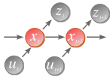
\includegraphics[width = 0.3\textwidth]{logo.png} % Just THIS!!!
    \end{center}
\end{figure}

\vspace*{10mm}
\normalfont\large
\texttt{MRPT}\\
Mobile Robot Programming Toolkit\\
Version: \MRPTVERSION

\vspace*{10mm}

\horrule{0.5pt} \\[0.4cm] % Thin top horizontal rule
\LARGE graphslam-engine: execute graphSLAM using rawlog files in MRPT
\horrule{2pt} \\[0.5cm] % Thick bottom horizontal rule
\vspace*{10mm}

\normalfont\large
Nikos Koukis\\
nickkouk@gmail.com\\
National Technical University of Athens\\
\vspace*{10mm}
\vfill

Document build: \today


\end{center}
\end{titlepage}

\newpage
\tableofcontents
\listoffigures
%\lstlistoflistings
\blankpage
\begin{abstract}

Current report delves into the new capabilities of mrpt-graphslam library and
provides a complete guide for using the \texttt{graphslam-engine} application.
More specifically it deals with the following:

\begin{itemize*}
    \item Description of major mrpt-graphslam library structure and concepts (e.g.\
        CGraphSlamEngine, decider, optimizers classes)
    \item \texttt{graphslam-engine} usage information (e.g.\ command line arguments)
\end{itemize*}

The extension of mrpt-graphslam library as well as the coding of the
corresponding graphslam-engine application was implemented as part of the
\textit{Google Summer of Code 2016 program}.

\end{abstract}

\printnomenclature[0.5in] % print the nomenclature
\newpage
\section{Introduction to graphSLAM}
An autonomous robot needs to address two critical problems to survive and
navigate within its surroundings: mapping the environment and finding its
relative location within the map. Simultaneous localization and mapping
(SLAM) is a process that aims to localize an autonomous mobile robot in a
previously unexplored environment while constructing a consistent and
incremental map of its environment~\cite{Saeedi2016}.
While filtering methods (extended Kalman filtering, information-form
filtering, particle filtering) used to dominate the SLAM literature, recently
(~2006) graph-based approaches have made a comeback. Introduced by Lu and
Milios in 1997~\cite{Lu1994} graph-based approaches formulate SLAM as a least-squares
minimization problem.

\section{Application Usage}

Aim of the app is to perform 2D graphSLAM: Robot localizes itself in the
environment while, at the same time builds a map of that environment. App
currently executes SLAM using MRPT rawlog files (both MRPT rawlog formats are
supported) as input which should contain (some of) the following observation
types:

\begin{itemize*}
    \item CObservationOdometry
    \item CObservation2DRangeScan
    \item CObservation3DRangeScan\hfill\\
        Working with 3DRangeScans is currently in an experimental phase.
\end{itemize*}

The majority of the graphslam-engine parameters in each case should be
specified in an external~.ini file which is to be given as a command-line
argument. The following parameters can also be specified as command-line
arguments:

\begin{description*}
    \item[.ini-file [REQUIRED] ]\hfill\\
        Specify the .ini configuration file using the \texttt{-i},
        \texttt{-\--ini-file} flags.
        Configuration file parameters are read by the main CGraphSlamEngine
        class as well as the node/edge registration schemes, and the
        optimization scheme.
    \item[rawlog-file [REQUIRED] ]\hfill\\
        Specify the rawlog dataset file using the \texttt{-r},
        \texttt{-\--rawlog} flags.
    \item[ground-truth]\hfill\\
        Specify a ground truth file with \texttt{-g}, \texttt{-\--ground-truth} flags. Ground truth
        has to be specified if user has set visualize\_slam\_metric or
        visualize\_ground\_truth to true in the .ini file, otherwise an
        exception is raised.
    \item[node/edge registration deciders]\hfill\\
        Specify the node registration or/and edge registration decider
        classes to be used using \texttt{-n}, \texttt{-\--node-reg},
        \texttt{-e}, \texttt{-\--edge-reg} flags. If not
        specified the default CFixedIntervalsNRD, CICPCriteriaERD are used
        as node and edge registration decider schemes respectively.
    \item[optimizer class to be used]\hfill\\
        Specify the class to be used for the optimization of the pose-graph
        using the \texttt{-o}, \texttt{-\--optimizer} flags. Currently the only supported
        optimization scheme is Levenberg-Marquardt non-linear graph
        optimization defined in
\href{http://reference.mrpt.org/devel/group\_\_mrpt\_\_graphslam\_\_grp.html\#ga022f4a70be5ec7c432f46374e4bb9d66}{optimize\_graph\_spa\_levmarq}. If not specified, the default CLevMarqGSO is used.
\end{description*}

Furthermore, application offers the following capabilities to the user:
\begin{itemize*}
    \item Support of both kinds of MRPT rawlog formats,
        action-observations and observation-only format. However, users should
        also make sure that the deciders/optimizer classes that are to be used
        also support the rawlog format that they are interested in.
    \item Visual inspection of graphSLAM execution. Apart from others the
        visualization window can be configured, by the user, to include the
        following:
        \begin{itemize*}
            \item graphSLAM estimated robot trajectory
            \item Odometry-only trajectory
            \item ground-truth trajectory (if the corresponding ground-truth is
                available
            \item Current robot 2D laser scan footprint
            \item Draft version of the map
            \item Currently constructed graph as edges between the registered
                nodes
        \end{itemize*}

    \item Hotkeys support for triggering various visualization features on/off.
        \footnote{Any registration decider / optimizer can get notified of
            keyboard/mouse events and can modify the visuals when these occur.
            For more on this see the corresponding
            \href{http://reference.mrpt.org/devel/classmrpt\_1\_1graphslam\_1\_1\_c\_registration\_decider\_or\_optimizer.html\#a3d8445d2382e282f3a03edfa686c6e22}{method}}

\end{itemize*}

\subsection{command-line arguments}

The available command line argument are also listed below, along with a
description of their usage:

\verbatiminput{./input/application_cmd_synopsis.txt}
\verbatiminput{./input/application_cmd_options.txt}

\subsection{Application output}
By default graphslam-engine execution generates an output directory by the name
\textit{graphslam\_results} within the current working directory. The output directory
contains the following files:

\begin{description*}
    \item[CGraphSlamEngine.log]\hfill\\
    Logfile containing the activity of the CGraphSlamEngine class instance.
    Activity involves output logger messages, time statistics for critical
    parts of the application, and summary statistics about the constructed
    graph (e.g. number of registered nodes, edges).
    \item[node\_registrar.log, edge\_registrar.log, optimizer.log]\hfill\\
    Logfiles containing the activity of the corresponding class instances. File
    contents depend on the implementation of the corresponding classes but in
    most cases they contain output logger messages, time statistics for
    critical parts of the class execution.
    \item[output\_graph.graph]\hfill\\
    File contains the constructed graph in the VERTEX/EDGE format. The latter
    can be visualized using the MRPT graph-slam application for verification
    reasons.
    For more information on this, consult the following pages:
    \begin{itemize*}
        \item \url{http://www.mrpt.org/Graph-SLAM\_maps}
        \item \url{http://www.mrpt.org/list-of-mrpt-apps/application-graph-slam/}
    \end{itemize*}

    \item[output\_scene.3DScene]\hfill\\
        File contains the 3DScene that was generated in the end of the
        graphslam-engine execution. The latter can be visualized using the MRPT
        SceneViewer3D tool.
        For more information on this, see:
        \url{http://www.mrpt.org/list-of-mrpt-apps/application-sceneviewer3d/}

        \vspace*{10mm}
        \ul{\textit{Note:}} File is generated only when the visualization of the
        graph construction is enabled in the .ini configuration file. See .ini
        parameters as well as the \texttt{-\--disable} flag for more on this.

    \item[SLAM\_evaluation\_metric.log]\hfill\\
        File contains the differences between the estimated trajectory increments
        and the corresponding ground-truth increments and can be used to verify and
        evaluate the performance of the SLAM algorithm. For more information on the
        metric, see \cite{Burgard2009}
        
        \ul{\textit{Note:}} File is generated only when the ground-truth of the corresponding
        dataset is given.
\end{description*}

\ul{\textit{Note:}} In case a directory named graphslam\_results, generated during a
previous execution, already exists, it is, by default, overwritten. If this is
not the desired behavior, user can set the user\_decides\_about\_output\_dir
.ini parameter to true so that they are asked about this naming conflict during
program execution.

\section{Library Design}
In this section insight into the graphslam-engine application - and corresponding library - is provided.

CGraphSlamEngine is the main class executing graphslam. CGraphSlamEngine
delegates most of the graph manipulation tasks to node/edge registration
deciders and optimizer classes. This makes up for independence between the
different tasks as well as for a reconfigurable setup, as the user can select
to use different decider/optimizer classes depending on the situation. Users
can also write their own decider/optimizer classes by inheriting from one of
the
\href{http://reference.mrpt.org/devel/classmrpt_1_1graphslam_1_1deciders_1_1_c_node_registration_decider.html}{CNodeRegistrationDecider},
\href{http://reference.mrpt.org/devel/classmrpt_1_1graphslam_1_1deciders_1_1_c_edge_registration_decider.html}{CEdgeRegistrationDecider}, \href{http://reference.mrpt.org/devel/classmrpt_1_1graphslam_1_1optimizers_1_1_c_graph_slam_optimizer.html}{CGraphSlamOptimizer}
interfaces depending on what part they want to implement.

\subsection{Registration Deciders}
The registration decider classes are divided into node and edge registration
deciders. The former are responsible of adding new nodes in the graph while the
latter add additional edges between already registered graph nodes. These nodes can
be consecutive or non-consecutive.

\subsubsection{Node Registration Deciders (NRD)}
Node registration decider schemes add nodes to the graph according to a
specific criterion. Node deciders should implement the methods defined in the
CNodeRegistrationDecider abstract class. The latter provides the basic methods
that have to exist in every node registration decider class and which are
called from the main CGraphSlamEngine instance.  For an example of inheriting
from this class see
\href{http://reference.mrpt.org/devel/classmrpt_1_1graphslam_1_1deciders_1_1_c_fixed_intervals_n_r_d.html}{CFixedIntervalsNRD}.


Currently two specific node registration schemes have been implemented:
\begin{itemize*}
    \item \href{http://reference.mrpt.org/devel/classmrpt_1_1graphslam_1_1deciders_1_1_c_fixed_intervals_n_r_d.html}{CFixedIntervalsNRD} \hfill\\
    Decider registers a new node in the graph if the distance or the angle
    difference with regards to the previous registered node surpasses a
    corresponding fixed threshold. Decider makes use only of the
    CObservationOdometry instances in the rawlog file.
    \item \href{http://reference.mrpt.org/devel/structmrpt_1_1graphslam_1_1deciders_1_1_c_i_c_p_criteria_n_r_d_1_1_t_params.html}{CICPCriteriaNRD} \hfill\\
    Decider registers a new node in the graph if the distance or the angle
    difference with regards to the previous registered node surpasses a
    corresponding fixed threshold. Decider measures the distance from the
    current position to the previous registered node using ICP (i.e. matches
    the current range scan against the range scan of the previous node). In
    case of noisy 2D laser scans, decider can also use odometry information to
    locally correct and smoothen the robot trajectory. Decider makes use of
    2DRangeScans or 3DRangeScans.
\end{itemize*}


\ul{\textit{Note:}} As a naming convention, all the implemented node registration deciders are
suffixed with the NRD acronym.
For more information on this see the

\href{http://reference.mrpt.org/devel/classmrpt_1_1graphslam_1_1deciders_1_1_c_node_registration_decider.html}{node
registration deciders interface}

\subsubsection{Edge Registration Deciders (ERD)}

Edge registration decider schemes add edges between already added nodes in the
graph according to a specific criterion. Edge deciders should implement the
methods defined in CEdgeRegistrationDecider abstract class.
CEdgeRegistrationDecider provides the basic methods that have to exist in every
edge registration decider class. For an example of inheriting from this class
see CICPCriteriaERD.

Currently two specific edge registration schemes have been implemented:

\begin{itemize*}
    \item \href{http://reference.mrpt.org/devel/structmrpt_1_1graphslam_1_1deciders_1_1_c_i_c_p_criteria_e_r_d_1_1_t_params.html}{CICPCriteriaERD} \hfill\\
		Register new edges in the graph with the last inserted node. Criterion for
		adding new edges should be the goodness of the
		candidate ICP edge. The nodes for ICP are picked based on the distance from the
		last inserted node. Decider makes use of 2DRangeScans or 3DRangeScans.

    \item \href{http://reference.mrpt.org/devel/classmrpt_1_1graphslam_1_1deciders_1_1_c_loop_closer_e_r_d.html}{CLoopCloserERD}\hfill\\
		Evaluate sets of potential loop closure edges in the graph based on their
		pairwise consistency matrix.Decider first splits the graph into partitions
		based on the 2D laser scans of the nodes and then searches for potential loop
		closure edges within the partitions. Goal is to register only a subset of the
		potential loop closure edges that maximally agree with each other. Decider is
		implemented based on \cite{Blanco2006}, \cite{Olson2009}

\end{itemize*}

\ul{\textit{Note:}} As a naming convention, all the implemented edge
registration deciders are suffixed with the ERD acronym.

For more information on this see the
\href{http://reference.mrpt.org/devel/classmrpt_1_1graphslam_1_1deciders_1_1_c_edge_registration_decider.html}{edge
registration deciders interface}

\subsection{graphSLAM Optimizers (GSO)}

Optimizer classes optimize an already constructed graph so that the registered
edges maximally agree with each other. Optimizer schemes should implement the
methods defined in
\href{http://reference.mrpt.org/devel/classmrpt_1_1graphslam_1_1optimizers_1_1_c_graph_slam_optimizer.html}{CGraphSlamOptimizer}
abstract class. For an example of inheriting from this class see
\href{http://reference.mrpt.org/devel/classmrpt_1_1graphslam_1_1optimizers_1_1_c_lev_marq_g_s_o.html}{CLevMarqGSO}.

\ul{\textit{Note:}} As a naming convention, all the implemented optimizer
classes are suffixed with the GSO acronym.

For more information on this see the
\href{http://reference.mrpt.org/devel/classmrpt_1_1graphslam_1_1optimizers_1_1_c_graph_slam_optimizer.html}{graphSLAM optimizers interface}

\subsection{Notable links}
Below important links for the library/application are provided:
\begin{itemize*}
    \item \href{http://www.mrpt.org/list-of-mrpt-apps/application-graphslamengine/}{graphslam-engine
        - Application page}
    \item \href{https://www.youtube.com/watch?v=Pv0yvlzrcXk}{Demonstration video}
    \item \href{http://reference.mrpt.org/devel/structmrpt_1_1graphslam_1_1_c_graph_slam_engine_1_1_t_r_g_b_d_info_file_params.html}{CGraphSlamEngine documentation}
    \item \href{http://reference.mrpt.org/devel/classmrpt_1_1graphslam_1_1_c_registration_decider_or_optimizer.html}{Registration Deciders / Optimizers documentation}
    \item \href{https://github.com/MRPT/GSoC2016-discussions/issues/2#}{GSoC 2016
        graphslam-engine discussion}
    \item Directory of ~.ini sample files: \url{../../share/mrpt/config_files/graphslam-engine/}
    \item Directory of demo datasets: \url{../../share/mrpt/datasets/graphslam-engine-demos/}

\end{itemize*}

\section{Further Improvements}
As of now, the mrpt-graphslam library is still under active development. A list of
features that have been scheduled for implementation are listed below:

\begin{itemize*}
    \item Cleanup and Fix code bugs
    \item Integrate with ROS --- Add support for online execution
    \item Add support for multi-robot graphSLAM
    \item Add nodes in the graph in an adaptive fashion
    \item Implement node reduction scheme
    \item Add support for visual sensors (e.g.\ working with point features as SIFT)
    \item Integrate with 3rd party optimization libraries
\end{itemize*}

For more details on the progress of the aforementioned improvements, see the
corresponding \href{https://github.com/MRPT/mrpt/milestone/9}{github milestone}



%%----------------------------------------------------------------------------------------
%%  BIBLIOGRAPHY
%%----------------------------------------------------------------------------------------
\newpage
\nocite{*}
\bibliographystyle{ieeetr}
\bibliography{./bibliography/stachniss_tutorial,%
              ./bibliography/consistent_observations.bib,%
              ./bibliography/olson_loop_closing,%
              ./bibliography/tutorial_se3_transformation,%
              ./bibliography/lu_milios.bib,%
              ./bibliography/saeedi_review.bib,%
              ./bibliography/comparison_of_SLAM_algorithms.bib}

\end{document}
